% =======================================================
% ============== Preamble ==================
% =======================================================
\documentclass[12pt,a4paper]{article} %Optional = twoside

\usepackage[english]{babel}
\usepackage[utf8]{inputenc}
\usepackage[T1]{fontenc}
\usepackage{amsmath}
\usepackage{amssymb}
\usepackage{gauss}
\usepackage{physics}
\usepackage{siunitx} %\si{} giver ordentlige enheder
\usepackage{caption}			%Tillader costum figurtekster
\usepackage[pdftex]{graphicx}	% Gør det muligt at inkludere grafik (bl.a. png og jpg) i dokumentet.
\usepackage{lastpage}			% Gør det muligt at skrive sidetallet af den sidste side.
\usepackage[textfont={rm, it}, labelfont={bf}]{caption}	% Definer hvordan figur tekster ser ud.
\usepackage{gensymb}			% Tilføjer ekstra symbol som grader celsius.
% Aktiverer todonotes pakken
\usepackage[bordercolor=gray!20,backgroundcolor=blue!10,textsize=footnotesize]{todonotes}
%\setlength{\marginparwidth}{0.6cm}	%Fix til brud ved twoside

\usepackage{icomma}				% Gør brug af komma som decimalseperator mulig.
\usepackage{pdfpages}			%Gør det muligt at indsætte PDF
\usepackage{cancel}
\usepackage{float}
\usepackage{slashed}
\usepackage{listings,xcolor}
\usepackage{setspace}
\usepackage{feynmp-auto}
\usepackage{hyperref}
\usepackage{neuralnetwork}

% ============== Setting up listings =========================
\definecolor{codegreen}{rgb}{0,0.6,0}
\definecolor{codegray}{rgb}{0.5,0.5,0.5}
\definecolor{codepurple}{rgb}{0.58,0,0.82}
\definecolor{backcolour}{rgb}{0.95,0.95,0.92}
\lstdefinestyle{mystyle}{
	backgroundcolor=\color{backcolour},   
	commentstyle=\color{codegreen},
	keywordstyle=\color{magenta},
	numberstyle=\tiny\color{codegray},
	stringstyle=\color{codepurple},
	basicstyle=\ttfamily\footnotesize,
	breakatwhitespace=false,         
	breaklines=true,                 
	captionpos=b,                    
	keepspaces=true,                 
	numbers=left,                    
	numbersep=5pt,                  
	showspaces=false,                
	showstringspaces=false,
	showtabs=false,                  
	tabsize=2
}
\lstset{style=mystyle}
% ============== Setting up fancy headers ... =========================
\usepackage{fancyhdr}
\pagestyle{fancy}
\renewcommand{\sectionmark}[1]{\markright{\thesection.\ #1}}
\lhead{\korttitel}
\chead{\dato}
\rhead{\navn}
\fancyfoot[RE,LO]{\kursus}
\cfoot{}
\fancyfoot[LE,RO]{Page \thepage\ of \pageref{LastPage}}
\renewcommand{\headrulewidth}{0.5pt}
\renewcommand{\footrulewidth}{0.5pt}

\fancypagestyle{plain}{%
	\renewcommand{\headrulewidth}{0pt}%
	\fancyhf{}%
	\fancyfoot[L]{\kursus}%
	\fancyfoot[R]{Page \thepage\ of \pageref{LastPage}}%
}

% Øg teksthøjden med 2 cm på alle sider
\addtolength\textheight{2cm}
\addtolength\topmargin{-1cm}
\addtolength\marginparwidth{1.5cm}
\addtolength\headheight{1.6pt}

\makeindex

% ============== Various options =================================
\numberwithin{equation}{section}
\setlength{\jot}{2ex}

% ============== Shothand =================================
\newcommand{\gamfa}[1]{\frac{1}{\sqrt{1-\frac{#1^2}{c^2}}}}
\newcommand{\gamfain}[1]{{\sqrt{1-\frac{#1 ^2}{c^2}}}}
\newcommand{\emf}{\mathcal{E}}

\newcommand{\en}[1]{\ \text{#1}}
\newcommand{\paa}[1]{\left(#1\right)}
\newcommand{\pd}{\partial}


% ============== Dokument egenskaber =============================
\newcommand{\titel}{Advanced machine learning}
\newcommand{\korttitel}{Lecture Notes}
\newcommand{\dato}{\today}
\newcommand{\navn}{Mattias Ermakov Thing}
\newcommand{\kursus}{CP3 Masterclass}

\title{\titel}
\author{\navn}
\date{\dato}

\begin{document}
	% ==================================================================
	% ====== Hovedafsnit=================================================
	% ==================================================================
	
	\maketitle

\section{Introduction, GitHub, and neural networks}\label{sec:lecture1}
	The first lecture is focused on establishing prerequisites and leveling out the playing field such that everyone is on the same page as we dive into the details in the following lectures. We take a look at structure of the course and GitHub where the course material is located. Then we will review the basics of neural network which will be the focus of this course.
	
	\subsection{Course overview}
		This course aim to introduce the students to various of methods of machine learning, primarily focused on neural networks and ways of training them. By the end of the course students should know about various types of neural network architectures and when to use a given architecture. We also look at ways to improve neural networks with physics guidance. The course consists of five two hour lectures with the following content:
		\begin{itemize}
			\item Introduction, GitHub, and neural networks
			\item Machine learning and methods of training
			\item Neural network architectures
			\item Physics guidance in neural networks
			\item TBD
		\end{itemize}
		Each lecture will come with relevant code and an exercise to prepare for the next lesson. Although the exercise is not mandatory, it is highly recommended to do as it will improve practical skills. The course material is available at: \url{https://github.com/CP3-Origins/advanced-machine-learning}. Beyond the lecture notes Google is your friend.
	
	\subsection{Prerequisites}
		This course will use Python and basic programming skills in this language is expected. To develop machine learning algorithms we will use \texttt{Keras} and \texttt{TensorFlow 2} \cite{chollet:2015keras, tensorflow:2015whitepaper}, which means students must have Python 3.8 installed or a newer version. The university provides the paid version of PyCharm as an IDE for Python, but you can use whatever for writing code.
		
		The required packages for the course can be found in the \texttt{requirement.txt} file in the \texttt{code} folder. From that directory you can install the packages with pip using: \texttt{pip install -r requirements.txt}
		
		The course material is located on GitHub (see the link in the course overview), and students can find the lecture notes in the \texttt{lecture\_notes} folder. The relevant code be found in the subfolders of the \texttt{code} folder.
		
		Students are expected to know calculus, linear algebra, and the basics of neural networks. This course builds on concepts from FY555 (Introduction to Python, machine learning and data handling for the physical sciences), but it is not necessary to have taken that course to follow.
		
	\subsection{Introduction to Git}
		All course material for this course is on GitHub and it is recommended you know how to access this material. GitHub is a developer platform using Git to manage projects. A link to the homepage of Git can be found here: \url{https://git-scm.com/}.
		
		Git is a free and open source distributed version control system. This means that it helps us manage versions of project and collaborate in an asynchronous fashion. Each contributor has a local version of the project, and can develop locally on that version, and then share changes in a controlled and versioned manner. Git is a key tool for code development and if you ever plan to work in IT, it is something you need to know. It can also be very useful for doing scientific work in groups if code is involved. Also, it allows you to save code and other files in the cloud as a backup. Two of the most popular platforms for using Git is GitHub and GitLab. In this course we use GitHub. Students are encourages to study Git and version control.
		
		There are five main commands you will need to use Git: \texttt{git clone}, \texttt{git pull}, \texttt{git add}, \texttt{git push}, and \texttt{git push}.
		
		To get started you need to download and install Git. Having installed Git you can clone the course repository. This can be done several ways:
		\begin{itemize}
			\item Using a Git plugin in your IDE
			\item With a \texttt{git clone} command in your terminal
			\item By downloading the repository as a zip file (not recommended)
		\end{itemize}
		If you just download the repository as a zip file, you an not leveraging Git. This method works if you simply want to download the course content, but will not teach you how to use Git.
		
		In the following we will consider how to work with Git using the terminal. Assume you want to download the course content from GitHub. Then you would go to the directory where you want to download the repository and execute the following command:\newline \newline
		\texttt{git clone git@github.com:CP3-Origins/advanced-machine-learning.git}
		\newline  \newline
		This will download the repository on your device. Since this course will be updated and improved throughout the course, there might be changes to the course. To update to the latest version you can use the following command anywhere inside the Git project by executing the \texttt{git pull} command.

		This will however not work, if you have locally modified a part of the repository, which you are trying to update. This is to avoid overwriting changes when merging the new file with your local files. In this case you need to resolve any merge issues, such that the file are merged in the desired way without having loosing any work due to file overwriting.
		
		If you plan to participate in exercises and develop your own networks, then it is recommended that you start by creating a fork of the repository. This will create a copy of the repository which is on your own GitHub account. The only downside is that you need to remember update your own fork to get the updates from the main repository on CP3. Other than that you can clone your forked repository and use pull to update your repository.
		
		Suppose you have made your own script with some neural network as part of an exercise, you can now upload that to your fork and save your changes to the cloud. In this case, if you loose your computer, you will still have everything from this course including any code you have created.
		
		To do this you need to push your code from you local machine to your fork on GitHub. To get an overview of file changes in the Git project, you can use the command \texttt{git status}. Then you can add the files you want to save using the command \texttt{git add <path/to/file>}. You can specify a folder or file which you want to add. You can execute \texttt{git add .} if you want all changes to be added. 
		
		Next, you need to commit the code to Git. This is for version control. Together with this it is recommended that you add a short note on what you change does. And example would be \texttt{git commit -m "Adds a network to model rainfall"}, where \texttt{-m} is the message flag and the part in double quotation is the commit message.
		
		Finally, you can use the push command to push the changes using the command \texttt{git push}. This will push your local changes to your fork and you should be able to see the changed if you open your repository on GitHub.
		
		The reason for using the fork is that it creates a personal copy for each student. We cannot have each student to save their work on the main course repository. This would also cause collisions if students used the same file names. You own your fork and you can invite colleagues to your participate if you want to work on the exercise together. 

	\subsection{Neural networks}
		Before going into a more thorough overview of machine learning (ML) methods, let us recall the basics of neural networks and look a implementing neural networks. In the next lecture we will get back to a general discussion of neural networks.
		
		\subsubsection{Theory}
			As the name suggest neural networks are composed of neurons similar to our brain. Any neuron network uses the same basic building block, the single neuron. In some applications such as in robots less than 100 may be sufficient \cite{nagler:2011}, whereas image classification networks may contain thousands of neurons \cite{lorente:2021}. Thus, to understand neural networks we should take our time to understand how they work. Neurons are fundamentally doing linear regression, and later we discuss how nonlinear behavior is obtained as this is key to the power of neural networks. As a simple example, one can consider a single neuron "network" shown in Figure \ref{fig:basicNN}. This "network" takes in three inputs, $x_i$, where $i=1,2,4$, and computes a predicted value $\hat{y}$. The word network is in quotation as one would need multiple interconnected neurons to properly talk of a network. 
			
			\begin{figure}
				\centering
				\begin{neuralnetwork}[height=4]
					\newcommand{\x}[2]{$x_#2$}
					\newcommand{\y}[2]{$\hat{y}_#2$}
					\inputlayer[count=3, bias=false, title=Input\\layer, text=\x]
					\outputlayer[count=1, title=Output\\layer, text=\y] \linklayers
				\end{neuralnetwork}
				\caption{A simple neural network with an input layer, and a single neuron in the output layer.}
				\label{fig:basicNN}
			\end{figure}
			
			In the case of this single neuron with three inputs shown in Figure \ref{fig:basicNN} the equation becomes,
			\begin{gather}
				z(x_i) = w_1 x_1 + w_2 x_2 + w_3 x_3 + b,
			\end{gather}
			where each input is associated with the weight $w_i$ which modulates the influence of the input, and then there is a bias term, $b$. This can be written in a compact matrix form as,
			\begin{gather}
				z_j(x_i) = 
				\begin{bmatrix}
					w_{11} & w_{21} & w_{31} \\
				\end{bmatrix}
				\begin{bmatrix}
					x_1\\
					x_2 \\
					x_3 \\
				\end{bmatrix}
				+
				\begin{bmatrix}
					b \\
				\end{bmatrix}
				= 
				w_{ij}x_i + b_j \cdot \vec{1},
			\end{gather}
			where an additional $j$ index is added to indicate the number of neurons, but since there is only one neuron it is redundant. The use of this index becomes apparent when considering a network like in Figure \ref{fig:lessbasicNN}, but with two fully connected output nodes, $j=2$. In this case, the equation would be,
			\begin{gather}
				z_j(x_i) = 
				\begin{bmatrix}
					w_{11} & w_{21} & w_{31} \\
					w_{12} & w_{22} & w_{32} \\
				\end{bmatrix}
				\begin{bmatrix}
					x_1\\
					x_2 \\
					x_3 \\
				\end{bmatrix}
				+
				\begin{bmatrix}
					b_1 \\
					b_2 \\
				\end{bmatrix}
				= 
				w_{ij}x_i + b_j \cdot \vec{1}.
			\end{gather}
			
			\begin{figure}
				\centering
				\begin{neuralnetwork}[height=4]
					\newcommand{\x}[2]{$x_#2$}
					\newcommand{\y}[2]{$\hat{y}_#2$}
					\inputlayer[count=3, bias=false, title=Input\\layer, text=\x]
					\outputlayer[count=2, title=Output\\layer, text=\y] \linklayers
				\end{neuralnetwork}
				\caption{A simple neural network with an input layer, and two neurons in the output layer.}
				\label{fig:lessbasicNN}
			\end{figure}
			
			This highlights the benefit of the notation with the weight matrix as $w_{ij}$, the input vector as $x_i$, and the bias vector as $b_j$. A technical note would be that, in practice, it is more efficient to skip the process of adding the bias terms explicitly. One can exploit the definition of matrix multiplication and write it as,
			\begin{gather}
				z_j(x_i) = 
				\begin{bmatrix}
					w_{11} & w_{21} & w_{31} & b_1\\
					w_{12} & w_{22} & w_{32} & b_2\\
				\end{bmatrix}
				\begin{bmatrix}
					x_1\\
					x_2 \\
					x_3 \\
					1 \\
				\end{bmatrix}
				= 
				w_{ij}x_i + b_j \cdot \vec{1}.
			\end{gather}
			
			From this we can then also consider more complex networks with hidden layers as in Figure \ref{fig:NNhidden}. In this case we would first compute the first the values at the hidden layers $z_1(x_i) = a_i $ and then we can use that result to compute that result $z_2(a_i) = \hat{y}$.
			\begin{figure}
				\centering
				\begin{neuralnetwork}[height=4]
					\newcommand{\hidden}[2]{$a_#2$}
					\newcommand{\x}[2]{$x_#2$}
					\newcommand{\y}[2]{$\hat{y}_#2$}
					\inputlayer[count=3, bias=false, title=Input\\layer, text=\x]
					\hiddenlayer[count=3, bias=false, title=Hidden\\layer, text=\hidden] \linklayers
					\outputlayer[count=1, title=Output\\layer, text=\y] \linklayers
				\end{neuralnetwork}
				\caption{A simple neural network with an input layer, a hidden layer, and a single neuron in the output layer.}
				\label{fig:NNhidden}
			\end{figure}
			
			A linear equation is not sufficient to produce complex nonlinear decision boundaries, therefore it is key to modify the result $z_j(x)$ such nonlinearity is achieved. This is very simply to prove, consider our simple network with one hidden layers. The math becomes,
			\begin{gather}
				\hat{y} = z_2(z_1(x_i)) = w_{i2}\paa{w_{i1}x_i + b_1 \cdot \vec{1}} + b_2 \cdot \vec{1}.
			\end{gather}
			The problem here is that while we have different weights and biases, due to the lack of nonlinearity, this hidden actually achieve nothing because we can redefine this equation to be just like a network without a hidden layer,
			\begin{gather}
				\hat{y} = z_2(z_1(x_i)) = \underbrace{w_{i2}w_{i1}x_i}_{w_{i1}x_i} + \underbrace{w_{i2}b_1 \cdot \vec{1} + b_2 \cdot \vec{1}b_1 \cdot \vec{1}}_{b_1 \cdot \vec{1}}.
			\end{gather}
			This is perfectly valid because the latter terms is nothing but a sum of trainable variable, which is nothing but a number, and then first part contains the input times two different weight, but again we can just redefine that as a single weight. Therefore, without any nonlinearity we can add an arbitrary number of hidden layers and achieve the equivalent of having no hidden layers.
			
			This is fixed using nonlinear activation functions, $a(z)$, such as the sigmoid function, $\sigma(x)$, and the rectifier linear (ReLu) function, $\rm{ReLu}(x)$. There are many more options, and it is up to the designer of the network to determine the best activation function. The activation function, $f$, can be applied on a per-neuron basis, but it is commonly applied across the layers,
			\begin{gather}
				a(z_j(x_i)) = f(w_{ij}x_i + b_j \cdot \vec{1}).
			\end{gather}
			Each layer of the neural network is generally computed in this way. One can then stack the layers, $a(z_j)^n$, where $n$ is the number of layers. Deep neural networks then have three layers or more, $n \ge 3$. The output of the neural network is then computed by iteratively computing the layers from input to output, with the previous layer being the input to the next layer.
			
		\subsection{Tensorflow and keras}
			For this course we will be using \texttt{Keras} and \texttt{TensorFlow 2} \cite{chollet:2015keras, tensorflow:2015whitepaper} to develop neural network. There are also other packages such as \texttt{PyTorch} \cite{paszke2017automatic} which you are free to use, but it will not be used in the example code of this course. At the end of the day it is all linear algebra, but there are some differences in the packages. In general \texttt{Keras} provides a more beginner-friendly interface, but we will introduce advanced features which can be done in both \texttt{TensorFlow} and \texttt{PyTorch}. Some of the exercises are will be suitable to do in \texttt{PyTorch} and you are welcome to do so.
			
			This weeks exercise is about introducing the basics of coding with \texttt{Keras} and \texttt{TensorFlow 2}. This example has also been used in FY555, but in this course we will consider a different exercise.
			
			
			
			
		
		
\section{Machine learning and methods of training}
	In this lecture we look at machine learning in a broader perspective to get a feeling for the different methods which one can use. Then we focus in on neural networks and deep learning, before looking at methods of training neural networks.
	
	\subsection{Machine learning}
		Before we go into advanced concepts of neural networks, we better take a step back to understand the bigger picture. What is the difference between machine learning (ML), artificial intelligence (AI), neural networks (NNs), and deep learning (DL)?
		
		As it turns out, neural networks is an outlier in this list. Neural networks is a particular method of machine learning, just like linear regression and decision trees. 
		\begin{figure}
			\centering
			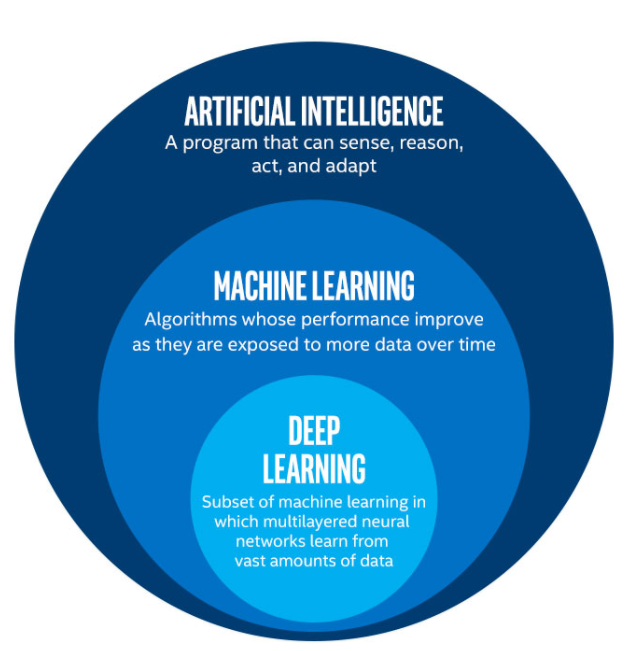
\includegraphics[width=0.7\linewidth]{figs/ai}
			\caption{An overview of the connection between AI, ML, DL. Note that neural networks are not mentioned.}
			\label{fig:ai}
		\end{figure}
		
		As shown in Figure \ref{fig:ai}, AI is the overarching name for algorithms that aim to imitate some kind of intelligence. A very simple AI that does not use any kind of fancy ML methods would be something like the following code:
		\begin{lstlisting}[language=Python]
if temperature > 20: 
	return 0
else:
	return 1
		\end{lstlisting}
		This example code is very simple, but it shows a simple AI algorithm which for example could be used to control temperature based on some temperature reading. One can make a more complex logic, but this is how one can make basic AI algorithms, and such algorithms have often been used in the past for various of applications to control sensors or bots in computer games.
		
		Machine learning is a more advanced subset of AI methods where the algorithm can learn from data. Such algorithms do not require developers to hard code logic into the algorithms, as the algorithm will create its own logic after been trained on data. For complex methods such as neural networks it leads to the black box issue, that the developer does not understanding how the algorithm makes its decisions, but can merely try to assert if the decision is correct or not.
		

% -------------------------------------------------------------------
% Bibliography
% -------------------------------------------------------------------
\bibliographystyle{plain} % We choose the "plain" reference style
\bibliography{lecture_notes} % Entries are in the refs.bib file

\end{document}
